\documentclass[a4paper,12pt]{article}

\usepackage[utf8]{inputenc}
\usepackage[slovene]{babel}
\usepackage{graphicx}
\usepackage{siunitx}
\usepackage{amsmath}
\usepackage{commath}
\usepackage{booktabs}
\usepackage{url}
\usepackage{caption}
\usepackage{subcaption}
\usepackage{tikz}
\usepackage{multirow}
\usepackage{physics}
\usepackage[top=1.1in, bottom=1.3in, left=1.25in, right=1.25in]{geometry}

\renewcommand{\vec}[1]{\mathbf{#1}} % bold vectors
\newcommand{\sgn}{\operatorname{sgn}}

\begin{document}

\begin{titlepage}
\begin{center}
{\large \sc Univerza v Ljubljani \\
Fakulteta za matematiko in fiziko}

\vspace{5cm}

{\Large Rok Kuk\\}
\vspace{10mm}
{\bf \Large Precesija Lunine orbite}\\
\vspace{25mm}
{\large Zaključna naloga v sklopu predmeta \\
Računalniška orodja v fiziki}\\

\vfill

{\normalsize \sc Akademsko leto 2018/2019}
\end{center}
\end{titlepage}

\newpage
\section{Uvod}

Z izračunom dinamike Sonca, Zemlje in Lune želimo določiti periodo precesije 
vozelne črte Lunine tirnice in njene dolge osi ter ugotoviti, kaj vpliva na 
hitrost precesije.

\subsection{Precesija vozelne črte}
Vozelna črta je zveznica presečišč Lunine tirnice z ekliptiko. Precesija 
vozelne črte pomeni rotacijo vozelne črte v ekliptiki in s tem rotacijo
ravnine Lunine tirnice. Njena perioda je \SI{6798.38}{dni}~\cite{nasassd}.
\begin{figure}[h!]
    \centering
    \includegraphics[scale=0.48]{slikep/nodal-precession.png}
    \caption{Precesija vozelne črte. Slika na desni prikazuje stanje dve leti 
    pozneje. Ni v merilu. Na shemi je predpostavljeno, da je Lunina tirnica 
    elipsa, čeprav zaradi precesije ni povsem eliptična 
    (slika~\ref{fig:apsidal}).~\cite{nodal}}
\end{figure}

\subsection{Precesija dolge osi}
Apogej je točka v kateri je Luna v svoji tirnici najbolj oddaljena od Zemlje,
perigej pa točka v kateri je najbližje Zemlji. Dolga os je zveznica med apogejem 
in perigejem. Precesija dolge osi pomeni rotacijo dolge osi v ravnini Lunine 
tirnice. Njena perioda je \SI{3231.50}{dni}~\cite{nasassd}.
\begin{figure}[h!]
    \centering
    \includegraphics[scale=0.63]{slikep/apsidal-precession.png}
    \caption{Lunina tirnica. Shema ni v merilu, precesija in ekscentričnost 
    sta pretirani. Apogej, Zemlja in perigej ne ležijo na isti premici, saj se 
    zaradi precesije apogej rahlo zamakne glede na  apogej, ki bi ga dobili, če
    bi narisali elipso, ko je Luna v perigeju.}
    \label{fig:apsidal}
\end{figure}

\newpage

\subsection{Predpostavke modela}
Do precesije Lunine tirnice pride zaradi gravitacijskega vpliva Sonca in drugih 
planetov na Luno, izbočenosti Zemlje ob ekvatorju ter relativističnih 
efektov~\cite{apsidal}. Glavni vzrok za precesijo Lune je gravitacijska sila 
Sonca, ki povzroča navor na Lunino tirnico, saj je glede na ekliptiko nagnjena 
za $\approx \SI{5.145}{\degree}$~\cite{nasassd}.

\vspace{1em}
\noindent
Da bo izračun dinamike sistema lažji, bomo uporabili sledeče predpostavke:
\begin{itemize}
    \item Edina sila, ki jo bomo upoštevali, je gravitacijska.
    \item Obravnavali bomo sistem Sonca, Zemlje in Lune. Vpliv ostalih teles 
    v Osončju bomo zanemarili.
    \item Sonce, Zemlja in Luna bodo točkasta telesa. S tem zanemarimo vpliv
    oblike Zemlje in Lune.
    \item Sonce bo mirovalo v izhodišču koordinatnega sistema. Ker ima Sonce 
    veliko večjo maso od sistema Zemlja-Luna \mbox{(\num{333000}-krat)}, 
    bomo zanemarili vpliva Zemlje in Lune na Sonce.
\end{itemize}

\newpage
\section{Izračun dinamike sistema}

\noindent
Pri izračunih uporabimo kartezični koordinatni sistem ICRF. Postavljen 
je tako, da je Sonce v izhodišču in da je XY-ravnina enaka ekliptiki ob času 
J2000 TDB. Osi so pozitivno orientirane. Os X je usmerjena proti pomladišču, 
os Z pa je pravokotna na XY-ravnino in ima pozitivno stran obrnjeno v smer 
Zemljinega severnega pola.

\begin{figure}[ht]
    \centering
    \includegraphics[scale=0.3]{slikep/eklipticni-koord-sistem.png}
    \caption{Postavitev osi koordinatnega sistema.}
\end{figure}

\noindent
Lego Sonca, Zemlje in Lune predstavimo s krajevnimi vektorji
\begin{equation*}
    \vec{r_S} =
    \begin{bmatrix}
        0 \\ 0 \\ 0
    \end{bmatrix},\ 
    \vec{r_Z} = 
    \begin{bmatrix}
        x_Z \\ y_Z \\ z_Z
    \end{bmatrix},\ 
    \vec{r_L} = 
    \begin{bmatrix}
        x_L \\ y_L \\ z_L
    \end{bmatrix}.
\end{equation*}
Telo z maso $m_1$ in krajevnim vektorjem $\vec{r_1}$ deluje na 
telo z maso $m_2$ in krajevnim vektorjem $\vec{r_2}$ s silo
\begin{equation*}
    \vec{F_{12}} (\vec{r_1},\vec{r_2}) = -\frac{G m_1 m_2}
    {\ \norm{\vec{r_2}-\vec{r_1}}^2} \cdot 
    \frac{\vec{r_2}-\vec{r_1}}{\: \norm{\vec{r_2}-\vec{r_1}}}.
\end{equation*}
Z uporabo drugega Newtonovega zakona in deljenjem z maso dobimo enačbe gibanja
Zemlje in Lune
\begin{eqnarray}
    \vec{\ddot{r}_Z} &=& -Gm_S\frac{\vec{r_Z}}{\ \norm{\vec{r_Z}}^3}
    -Gm_L\frac{\vec{r_Z-r_L}}{\ \norm{\vec{r_Z}-\vec{r_L}}^3}, \nonumber \\
    \vec{\ddot{r}_L} &=& -Gm_S\frac{\vec{r_L}}{\ \norm{\vec{r_L}}^3}
    -Gm_Z\frac{\vec{r_L}-\vec{r_Z}}{\ \norm{\vec{r_L}-\vec{r_Z}}^3}. \nonumber
\end{eqnarray}

\noindent
Označimo $\vec{v_Z} = \vec{\dot{r}_Z}$ in $\vec{v_L} = \vec{\dot{r}_L}$.
Stanje sistema lahko opišemo s koordinatami in komponentami hitrosti 
Zemlje in Lune
\begin{equation*}
    \left[x_Z, y_Z, z_Z, x_L, y_L, z_L, v_{Zx}, v_{Zy}, v_{Zz}, v_{Lx}, 
    v_{Ly}, v_{Lz}\right]. 
\end{equation*}

\noindent
Za reševanje diferencialnih enačb bomo uporabili \texttt{scipy.integrate.odeint} 
iz Pythonove knjižnice SciPy~\cite{odeint}. Tej funkciji moramo kot parameter 
podati funkcijo, ki izračuna odvod vsake spremenljivke stanja.

\noindent
Odvode izračunamo po komponentah
\begin{align*}
    &\dot{x}_Z = v_{Zx} & &\dot{x}_L = v_{Lx} \\
    &\dot{y}_Z = v_{Zy} & &\dot{y}_L = v_{Ly} \\
    &\dot{x}_Z = v_{Zz} & &\dot{z}_L = v_{Lz} \\
    &\dot{v}_{Zx} = - \frac{Gm_Sx_Z}{\: \norm{\vec{r_Z}}^3} - \frac{Gm_L(x_Z-x_L)}{\norm{\vec{r_Z}-\vec{r_L}}^3} & &\dot{v}_{Lx} = - \frac{Gm_Sx_L}{\: \norm{\vec{r_L}}^3} - \frac{Gm_Z(x_L-x_Z)}{\norm{\vec{r_L}-\vec{r_Z}}^3} \\
    &\dot{v}_{Zy} = - \frac{Gm_Sy_Z}{\: \norm{\vec{r_Z}}^3} - \frac{Gm_L(y_Z-y_L)}{\norm{\vec{r_Z}-\vec{r_L}}^3} & &\dot{v}_{Ly} = - \frac{Gm_Sy_L}{\: \norm{\vec{r_L}}^3} - \frac{Gm_Z(y_L-y_Z)}{\norm{\vec{r_L}-\vec{r_Z}}^3} \\
    &\dot{v}_{Zz} = - \frac{Gm_Sz_Z}{\: \norm{\vec{r_Z}}^3} - \frac{Gm_L(z_Z-z_L)}{\norm{\vec{r_Z}-\vec{r_L}}^3} & &\dot{v}_{Lz} = - \frac{Gm_Sz_L}{\: \norm{\vec{r_L}}^3} - \frac{Gm_Z(z_L-z_Z)}{\norm{\vec{r_L}-\vec{r_Z}}^3}
\end{align*}
Funkciji \texttt{odeint} podamo funkcijo, ki je definirana s predpisom
\begin{eqnarray}
    &\left[x_Z, y_Z, z_Z, x_L, y_L, z_L, v_{Zx}, v_{Zy}, v_{Zz}, v_{Lx}, v_{Ly}, 
    v_{Lz}\right]' = \nonumber \\ 
    &\left[v_{Zx}, v_{Zy}, v_{Zz}, v_{Lx}, v_{Ly}, v_{Lz}, \dot{v}_{Zx}, 
    \dot{v}_{Zy}, \dot{v}_{Zz}, \dot{v}_{Lx}, \dot{v}_{Ly}, 
    \dot{v}_{Lz}\right]. \nonumber
\end{eqnarray}
Funkcija \texttt{odeint} vrne seznam koordinat in komponent hitrosti Zemlje in 
Lune ob željenih časovnih intervalih. Programska koda je na voljo na portalu 
GitLab \cite{repo}.

Za reševanje diferencialnih enačb potrebujemo začetne pogoje, ki jih pridobimo
iz sistema Horizons~\cite{nasassd} in so zbrani v spodnji tabeli.
\begin{table}[ht]
    \centering
    \begin{tabular}{c c c}
        \toprule
        & Zemlja & Luna \\
        \midrule
        $x$ [\si{\astronomicalunit}] & \hspace{0.5em} \num{2.499646121224160e-01} & \hspace{0.5em} \num{2.476511762731858e-01} \\
        $y$ [\si{\astronomicalunit}] & \num{-9.773336829448052e-01} & \num{-9.765652528404914e-01} \\
        $z$ [\si{\astronomicalunit}] & \hspace{0.5em} \num{2.463574436805279E-05} & \hspace{0.5em} \num{2.077343737630762E-04} \\
        $v_x$ [\si{\astronomicalunit}/dan] & \hspace{0.5em} \num{1.638044451748829E-02} & \hspace{0.5em} \num{1.617465022148979E-02} \\
        $v_y$ [\si{\astronomicalunit}/dan] & \hspace{0.5em} \num{4.210082689617622E-03} & \hspace{0.5em} \num{3.626725674604836E-03} \\
        $v_z$ [\si{\astronomicalunit}/dan] & \num{-4.284581571560084E-07} & \hspace{0.5em} \num{3.388411287849449E-05} \\
        \bottomrule
    \end{tabular}
    \caption{Koordinate in komponente hitrosti Zemlje in Lune ob času 
    \mbox{JD 2458671.5 TDB} (7. julij 2019 00:00:00 TT). 
    Referenčna epoha: J2000}
\end{table}

\begin{table}[b]
    \centering
    \begin{tabular}{c c}
        \toprule
        dan & \SI{86400}{\second} \\
        leto & \SI{365.25}{dni} \\
        \si{\astronomicalunit} & \SI{149597870700}{\metre} \\
        $G$ & \SI{6.67408e-11}{\metre\cubed\per\kilo\gram\per\second\squared} \\
        $Gm_S$ & \SI{0.295912208285591100e-3}{\astronomicalunit\cubed\per dan \squared} \\
        $Gm_Z$ & \SI{0.888769244512563400e-9}{\astronomicalunit\cubed\per dan \squared} \\
        $Gm_L$ & \SI{0.109318945074237400e-10}{\astronomicalunit\cubed\per dan \squared} \\
        \bottomrule
    \end{tabular}
    \caption{Vrednosti konstant uporabljenih pri
    izračunih.~\cite{konstante,codata}}
\end{table}

\newpage
\subsection{Precesija vozelne črte}
Ekliptika v poljubnem trenutku ni povsem enaka ravnini XY, saj smo ravnino XY 
definirali kot ekliptiko ob času J2000, ekliptika pa se s časom spreminja. Da 
bi lahko poiskali presečišča Lunine tirnice s trenutno ekliptiko, jo moramo 
najprej določiti. Dovolj je, da izračunamo njeno normalo, saj poteka skozi 
izhodišče.

S funkcijo \texttt{odeint} izračunamo krajevni vektor Zemlje 
in Lune ter z njima krajevni vektor težišča sistema Zemlja-Luna ob časovnih 
intervalih z razmikom ene ure. Normalo ekliptike ob poljubnem času določimo 
tako, da prilagodimo ravnino točkam, ki jih določajo krajevni vektorji težišča 
180 dni pred danim časom in 180 dni po danem času. Namesto krajevnih vektorjev 
Zemlje uporabimo krajevne vektorje težišča, ker zaradi vpliva Lune Zemlja niha 
v smeri osi Z s periodo približno 27 dni. Ravnina, ki bi jo prilagodili 
Zemljini tirnici, bi zato bila odvisna od faze Lune v začetnih in končnih 
točkah. Temu se izognemo tako, da uporabimo vektorje težišča, ki ima periodo
nihanja v smeri osi Z eno leto.

Da bi ugotovili kdaj Luna prečka ekliptiko, moramo vedeti, ali je Luna v danem 
trenutku nad ali pod ravnino. Če je $\theta$ kot med normalo ekliptike 
$\vec{n}$ in krajevnim vektorjem Lune $\vec{r_L}$, velja
\begin{equation*}
    \vec{n} \cdot \vec{r_L} = \norm{\vec{n}}\ \norm{\vec{r_L}} \cos{\theta},
\end{equation*}
\begin{equation*}
\sgn(\cos(\theta))=\left\{
    \begin{array}{ll}
        {1} & { ;\ 0 < \theta < \frac{\pi}{2}} \\ 
        {-1} & { ;\ \frac{\pi}{2} < \theta < \pi}
    \end{array}\right.
\end{equation*}
Ker je $\norm{\vec{n}} > 0$ in $\norm{\vec{r_L}} > 0$, velja 
$\sgn(\vec{n}\cdot\vec{r_L}) = \sgn(\cos{\theta})$. Dobili smo funkcijo, ki
nam pove, ali je točka nad ali pod ravnino. 

Točka je nad ravnino (v smeri normale) natanko tedaj, ko je $\theta$ med $0$ 
in $\frac{\pi}{2}$ ter je $\sgn(\vec{n}\cdot\vec{r_L}) = 1$. Točka je pod 
ravnino (v smeri nasprotni normali) natanko tedaj, ko je $\theta$ med 
$\frac{\pi}{2}$ in $\pi$ ter je $\sgn(\vec{n}\cdot\vec{r_L}) = -1$. Da 
ugotovimo, ali je poljubna točka nad ravnino ali pod njo, moramo preveriti le, 
kakšen je predznak skalarnega produkta njenega krajevnega vektorja z normalo 
ekliptike.

Za vsak časovni interval izračunamo skalarni 
produkt normale ekliptike s krajevnim vektorjem Lune.
Nato določimo točke, pri katerih se predznak skalarnega produkta spremeni.
To so točke, v katerih Luna prečka ekliptiko -- dvižni in spustni vozli.

Vsakemu vozlu priredimo vektor $\vec{e_i}$ z izhodiščem v težišču sistema 
Zemlja-Luna, ki predstavlja smer vozelne črte. Vsakemu dvižnemu vozlu priredimo 
vektor v smeri proti vozlu, vsakemu spustnemu vozlu pa vektor v smeri, ki je 
nasprotna smeri od težišča do vozla (slika \ref{fig:nodal}).
Zaradi precesije se bo vektor vozelne črte vrtel okrog težišča. Definiramo
i-ti kot vozelne črte $\phi_i$ s kotom med prvim vektorjem vozelne črte 
$\vec{e_1}$ in i-tim vektorjem vozelne črte $\vec{e_i}$ v pozitivni smeri glede 
na trenutno normalo ekliptike
\begin{equation*}
    \cos{\phi_i} = \frac{\: \vec{e_1} \cdot \vec{e_i}}
    {\; \norm{\vec{e_1}} \ \norm{\vec{e_i}}}.
\end{equation*}
Želimo rešitve od 0 do \SI{360}{\degree}. V prvem in drugem kvardantu nam 
$\arccos$ da pravo rešitev za kot, v tretjem in četrtem pa moramo rešitev 
odšteti od $2\pi$, da dobimo željeni kot. Da ugotovimo, v katerem kvadrantu se
vektor $\vec{e_i}$ nahaja, si pomagamo z vektorskim produktom. Če je vektorski 
produkt $\vec{e_1} \times \vec{e_i}$ v smeri normale ekliptike, je $\vec{e_i}$ 
v prvem ali drugem kvardrantu, če pa je vektorski produkt v nasprotni smeri 
normale ekliptike, je $\vec{e_i}$ v tretjem ali četrtem kvadrantu. Kot prej
določimo smer vektorskega produkta s skalarnim produktom. Rešitev je torej
\begin{equation}
    \phi_i = \left\{
        \begin{array}{ll}
            \arccos{\frac{\: \vec{e_1} \cdot \vec{e_i}}
            {\; \norm{\vec{e_1}} \ \norm{\vec{e_i}}}} & 
            {;\ (\vec{e_1}\times\vec{e_i})\cdot\vec{n} \geq 0} \vspace{0.5em} \\
            2\pi - \arccos{\frac{\: \vec{e_1} \cdot \vec{e_i}}
            {\; \norm{\vec{e_1}} \ \norm{\vec{e_i}}}} & 
            {;\ (\vec{e_1}\times\vec{e_i})\cdot\vec{n} < 0}
        \end{array}
    \right.
    \label{eq:nodal-kot}
\end{equation}
Gledano iz smeri Zemljinega severnega pola, se vozelna črta vrti v smeri 
urinega kazalca, zato se bo kot $\phi_i$ zmanjševal.

\begin{figure}[ht!]
    \centering
    \includegraphics[scale=0.55]{slikep/nodes-luna.png}
    \caption{Lunina tirnica in smerna vektorja. Prvi smerni vektor vozelne črte 
    kaže od težišča sistema Zemlja-Luna do dvižnega vozla, drugi pa od težišča 
    v nasprotno smer spustnega vozla. Težišče sistema je zelo blizu Zemlje.}
    \label{fig:nodal}
\end{figure}

\newpage

\subsection{Precesija dolge osi}
Najprej moramo določiti točke, v katerih je Luna v apogeju in perigeju. S 
funkcijo \texttt{odeint} izračunamo krajevna vektorja Zemlje in Lune ob
časovnih intervalih z razmikom ene ure. S krajevnima vektorjema izračunamo 
razdaljo med telesoma. Določimo minimume in maksimume razdalje med Zemljo in
Luno pri vsakem obhodu. Dobimo časovne intervale, pri katerih je Luna v apogeju 
in perigeju vsakega obhoda
\begin{align*}
    \text{apogej:} \quad &\max \norm{\vec{r_Z}-\vec{r_L}}, \\
    \text{perigej:} \quad &\min \norm{\vec{r_Z}-\vec{r_L}}.
\end{align*}

\noindent
Vsakemu perigeju in apogeju priredimo vektor $\vec{f_i}$ z izhodiščem v težišču
sistema Zemlja-Luna, ki predstavlja smer dolge osi. Vsakemu perigeju priredimo
vektor v smeri proti perigeju, vsakemu apogeju pa priredimo vektor v 
smeri, ki je nasprotna smeri od težišča do apogeja.

\begin{figure}[h!]
    \centering
    \begin{minipage}[t]{.5\textwidth}
        \centering
        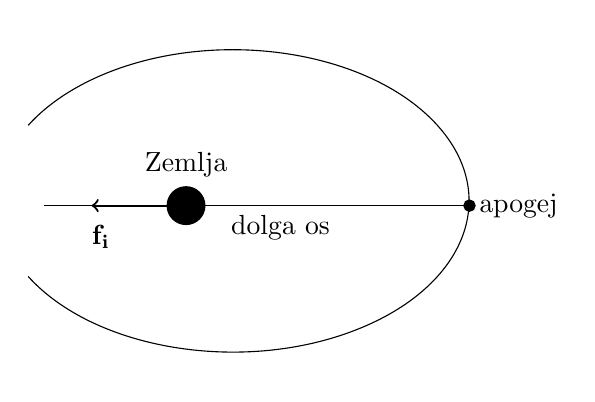
\begin{tikzpicture}[scale=1.2]
            \draw (-2.17,-0.75) arc(-150:150:2.5cm and 1.6cm);
            \draw [fill] (-0.5,0) circle [radius=0.2];
            \node [above] at (-0.5,0.2) {Zemlja};
            \draw[fill] (2.5,0) circle [radius=0.06];
            \node [right] at (2.5,0) {apogej};
            \draw (-2,0) -- (2.5,0);
            \node [below] at (0.5,0) {dolga os};
            \draw [thick, ->] (-0.5,0) -- (-1.5,0);
            \node [below] at (-1.4,-0.1) {$\vec{f_i}$};
        \end{tikzpicture}
        \begin{minipage}{0.8\textwidth}
            \caption{Lunina tirnica in smerni vektor, ko je Luna v apogeju.}
        \end{minipage}%
    \end{minipage}%
    \hfill
    \begin{minipage}[t]{.5\textwidth}
        \centering
        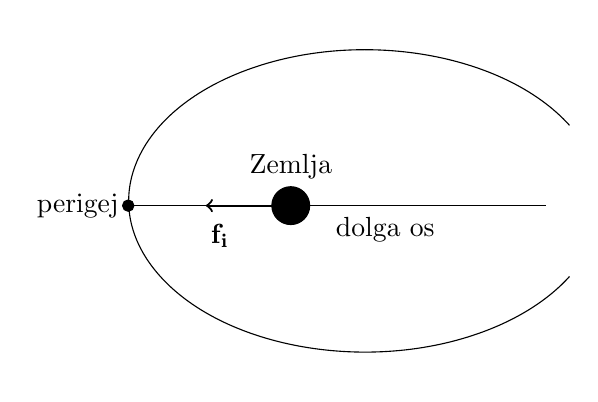
\begin{tikzpicture}[scale=1.2]
            \draw (1.25,1.37) arc(30:330:2.5cm and 1.6cm);
            \draw [fill] (-1.7,0.52) circle [radius=0.2];
            \node [above] at (-1.7,0.7) {Zemlja};
            \draw[fill] (-3.42,0.52) circle [radius=0.06];
            \node [left] at (-3.42,0.52) {perigej};
            \draw (-3.42,0.52) -- (1,0.52);
            \node [below] at (-0.7,0.5) {dolga os};
            \draw [thick, ->] (-1.7,0.52) -- (-2.6,0.52);
            \node [below] at (-2.45,0.43) {$\vec{f_i}$};
        \end{tikzpicture}
        \begin{minipage}{0.8\textwidth}
            \caption{Lunina tirnica in smerni vektor, ko je Luna v perigeju.}
        \end{minipage}
    \end{minipage}
\end{figure}

\noindent
Zaradi precesije se bo vektor dolge osi vrtel okrog težišča. Definiramo i-ti 
kot dolge osi $\gamma_i$ merjen v pozitivni smeri glede na trenutno normalo 
Lunine tirnice. Merimo ga od prvega vektorja dolge osi $\vec{f_1}$ do 
trenutnega vektorja dolge osi $\vec{f_i}$. Uporabimo podobno formulo kot za 
vektor vozelne črte \eqref{eq:nodal-kot}
\begin{equation*}
    \gamma_i = \left\{
        \begin{array}{ll}
            \arccos{\frac{\: \vec{f_1} \cdot \vec{f_i}}
            {\; \norm{\vec{f_1}} \ \norm{\vec{f_i}}}} & 
            {;\ (\vec{f_1}\times\vec{f_i})\cdot\vec{n_L} \geq 0} \vspace{0.5em} \\
            2\pi - \arccos{\frac{\: \vec{f_1} \cdot \vec{f_i}}
            {\; \norm{\vec{f_1}} \ \norm{\vec{f_i}}}} & 
            {;\ (\vec{f_1}\times\vec{f_i})\cdot\vec{n_L} < 0}
        \end{array}
    \right.
\end{equation*}

\noindent
Za izračun kota $\gamma_i$ potrebujemo normalo Lunine tirnice $\vec{n_L}$. Za
vsak vektor $\vec{f_i}$ jo izračunamo z vektorskim produktom med vektorjem,
ki kaže od težišča sistema Zemlja-Luna proti Luni in vektorjem, ki kaže od 
težišča sistema do lege Lune pred sedmimi dnevi.

Gledano iz smeri Zemljinega severnega pola, se vozelna črta vrti v nasprotni 
smeri urinega kazalca, zato se bo kot večal.

\newpage
\section{Rezultati}

\renewcommand{\figurename}{Graf}

\begin{figure}[ht!]
    \centering
    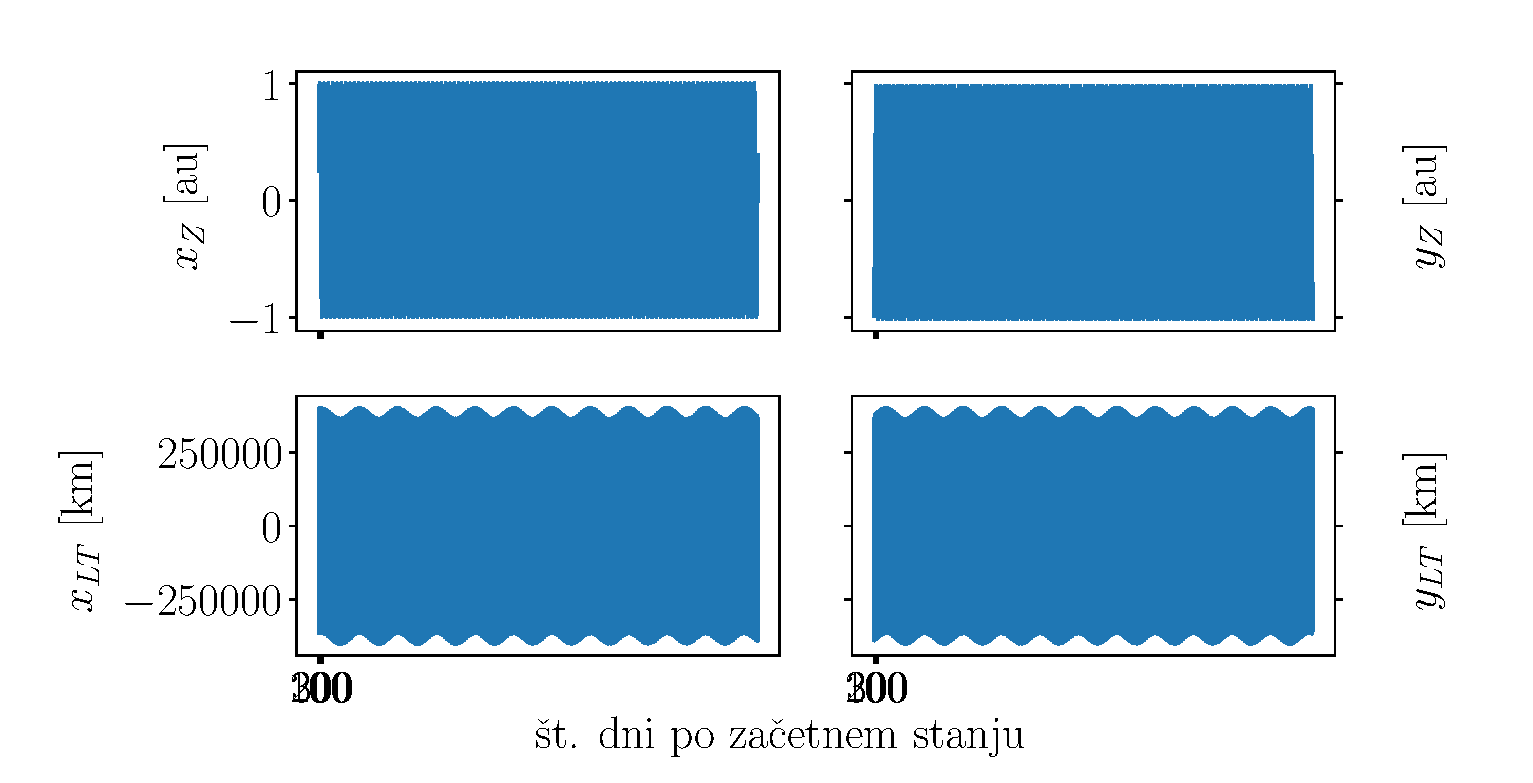
\includegraphics[scale=0.46]{slikep/koordinate.eps}
    \caption{Zgoraj: Zemljini koordinati $x$ in $y$ tekom enega leta. Spodaj: 
    Lunini koordinati $x$ in $y$ v koordinatnem sistemu z izhodiščem v težišču 
    sistema Zemlja-Luna tekom enega leta.}
    \label{fig:koordxy}
\end{figure}

\noindent
Iz grafa \ref{fig:koordxy} vidimo, da je gibanje Zemlje in Lune periodično.
Natančnost modela lahko ocenimo s primerjavo obhodnih časov Zemlje in Lune.
Ker se v 100 letih dolžini period ne spremenita bistveno (grafa 
\ref{fig:period-comp1}, \ref{fig:period-comp2}), izračunamo obhodna časa tako, 
da izračunamo povprečni periodi koordinate $x$ v 100 letih. Za koordinati $y$ 
in $z$ sta periodi v okviru napake enaki.

Za 100 obhodov Zemlje je potrebnih $\SI{36525.96}{dni}\pm\SI{0.04}{dneva}$, 
torej je Zemljin povprečen obhodni čas
$\SI{365}{dni}\ \SI{6}{\hour}\ \SI{14}{\minute}\pm\SI{1}{\minute}$. To je blizu,
a ne v okviru napake, referenčni vrednosti 
$\SI{365}{dni}\ \SI{6}{\hour}\ \SI{9}{\minute}$ \cite{nasassd}. Razlika med 
rezultatom in referenčno vrednostjo najverjetneje izvira iz neupoštevanja 
ostalih teles v Osončju.

Za 1350 obhodov Lune okrog težišča je potrebnih 
$\SI{36883.88}{dni}\pm\SI{0.04}{dneva}$, torej je Lunin povprečen obhodni čas
$\SI{27}{dni}\ \SI{7}{\hour}\ \SI{43}{\minute}\pm\SI{1}{\minute}$. To je v
okviru napake enako referenčni vrednosti
$\SI{27}{dni}\ \SI{7}{\hour}\ \SI{43}{\minute} \SI{5}{\second}$ \cite{nasassd}.

\begin{figure}[hb!]
    \centering
    \begin{minipage}[t]{.5\textwidth}
        \centering
        \includegraphics[scale=0.44]{slikep/obhodi-zemlja.eps}
        \begin{minipage}{0.8\textwidth}
            \caption{Dolžina posamezne periode Zemljine koordinate $x$.}
            \label{fig:period-comp1}
        \end{minipage}%
    \end{minipage}%
    \hfill
    \begin{minipage}[t]{.5\textwidth}
        \centering
        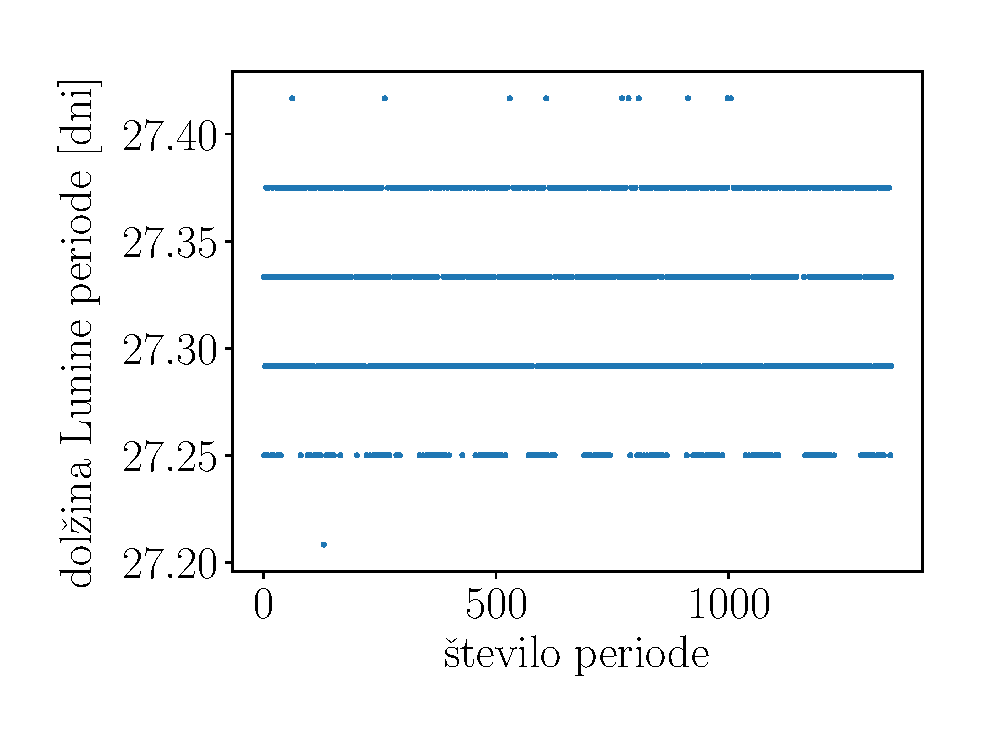
\includegraphics[scale=0.44]{slikep/obhodi-luna.eps}
        \begin{minipage}{0.9\textwidth}
            \caption{Dolžina posamezne periode Lunine kooridnate $x$ v
            težiščnem koordinatnem sistemu.}
            \label{fig:period-comp2}
        \end{minipage}
    \end{minipage}
\end{figure}

\newpage

\begin{figure}[ht]
    \centering
    \includegraphics[scale=0.53]{slikep/koordinatez.eps}
    \caption{Zemljina in Lunina koordinata $z$ tekom enega leta.}
    \label{fig:zemlja-luna}
\end{figure}

\noindent
Na grafu \ref{fig:zemlja-luna} opazimo, da ima nihanje Zemljine koordinate $z$ 
znotraj enega leta enako periodo kot nihanje Lunine koordinate $z$ znotraj 
enega leta in nasprotno fazo. To je posledica tega, da Zemlja in Luna (v prvem 
približku) krožita po elipsi okrog težišča sistema.

Natančnost modela preverimo tudi tako, da primerjamo odstopanje napovedi modela 
od napovedi sistema Horizons, ki upošteva tudi vplive drugih teles v Osončju.

\begin{figure}[hb!]
    \centering
    \begin{minipage}[t]{.5\textwidth}
        \centering
        \includegraphics[scale=0.44]{slikep/comparedelta.eps}
        \begin{minipage}{0.85\textwidth}
            \caption{Razlika med napovedjo modela in sistema Horizons za 
            Zemljino koordinato $x$.}
            \label{fig:comparedelta}
        \end{minipage}%
    \end{minipage}%
    \hfill
    \begin{minipage}[t]{.5\textwidth}
        \centering
        \includegraphics[scale=0.44]{slikep/comparedistance.eps}
        \begin{minipage}{0.85\textwidth}
            \caption{Razdalja med lego Zemlje kot jo napove model in lego
            Zemlje kot jo napove sistem Horizons.}
            \label{fig:comparedistance}
        \end{minipage}
    \end{minipage}
\end{figure}

\noindent
Na grafih \ref{fig:comparedelta} in \ref{fig:comparedistance} vidimo, da 
maksimalno odstopanje narašča približno linearno. Podobno je za ostale 
koordinate Zemlje in Lune. Znotraj ovojnice, ki jo določajo ekstremi, je 
odstopanje podobno sinusoidi s periodo enega leta, kar pomeni, da je pol leta 
koordinata $x$ modela manjša od napovedane s sistemom Horizons, pol leta pa 
večja. Enako velja tudi za koordinati $y$ in $z$. Če odstopanja koordinat med 
sabo primerjamo, ugotovimo, da lega Zemlje napovedana z modelom rahlo zaostaja 
za lego napovedano s Horizons.

Zaostajanje modela se ujema s tem, da je obhodni čas Zemlje v našem modelu
nekaj minut daljši od referenčne vrednosti. Odstopanje najverjetneje izhaja iz 
tega, da v modelu nismo upoštevali vpliva ostalih teles v Osončju, ki vplivajo
na Zemljino tirnico. Vpliva na Lunin obhodni čas najverjetneje nismo opazili 
zaradi premajhne natančnosti pri določanju Lunine lege, saj je obhodni čas
določen le na $\SI{1}{\minute}$ natančno.

\newpage 

\noindent
V modelu upoštevamo le gravitacijsko silo, ki je konservativna, zato bi se 
morala energija sistema ohranjati. Numerično napako lahko ocenimo z odstopanjem 
energije sistema od začetne energije. Skupna energija Sonca, Zemlje in Lune je
\begin{equation*}
    W = \frac{1}{2}m_Z\norm{\vec{v_Z}}^2 + \frac{1}{2}m_L\norm{\vec{v_L}}^2 -
    \frac{Gm_Sm_Z}{\norm{\vec{r_Z}}} - \frac{Gm_Sm_L}{\norm{\vec{r_L}}} 
    - \frac{Gm_Zm_L}{\: \norm{\vec{r_Z}-\vec{r_L}}}.
\end{equation*}

\begin{figure}[ht!]
    \centering
    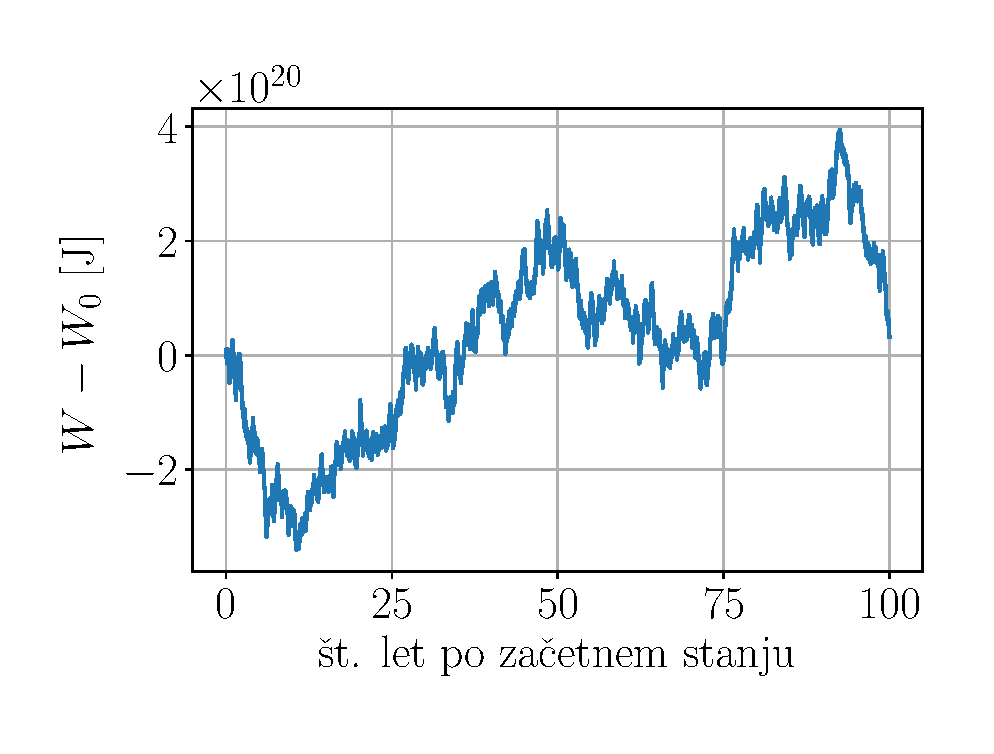
\includegraphics[scale=0.55]{slikep/energija.eps}
    \caption{Odstopanje energije sistema od začetne energije 
    $W_0=\SI{-2.7e33}{\joule}$.}
\end{figure}

\noindent
Pri uporabi funkcije \texttt{odeint} je bilo potrebno omejiti maksimalni
korak integracije, sicer je sistem opazno pridobival energijo in se je Luna
preveč oddaljila od Zemlje.

Odstopanje energije sistema je 13 redov velikosti manjše od energije sistema, 
zato sklepamo, da je vpliv numerične napake na rezultate zanemarljiv. Na 
spodnjih grafih vidimo, da sta tirnici Zemlje in Lune stabilni in da ostajajo 
ekstremi razdalj Zemlja-Luna in Zemlja-Sonce približno enaki.

\begin{figure}[h]
    \centering
    \begin{minipage}[t]{.5\textwidth}
        \centering
        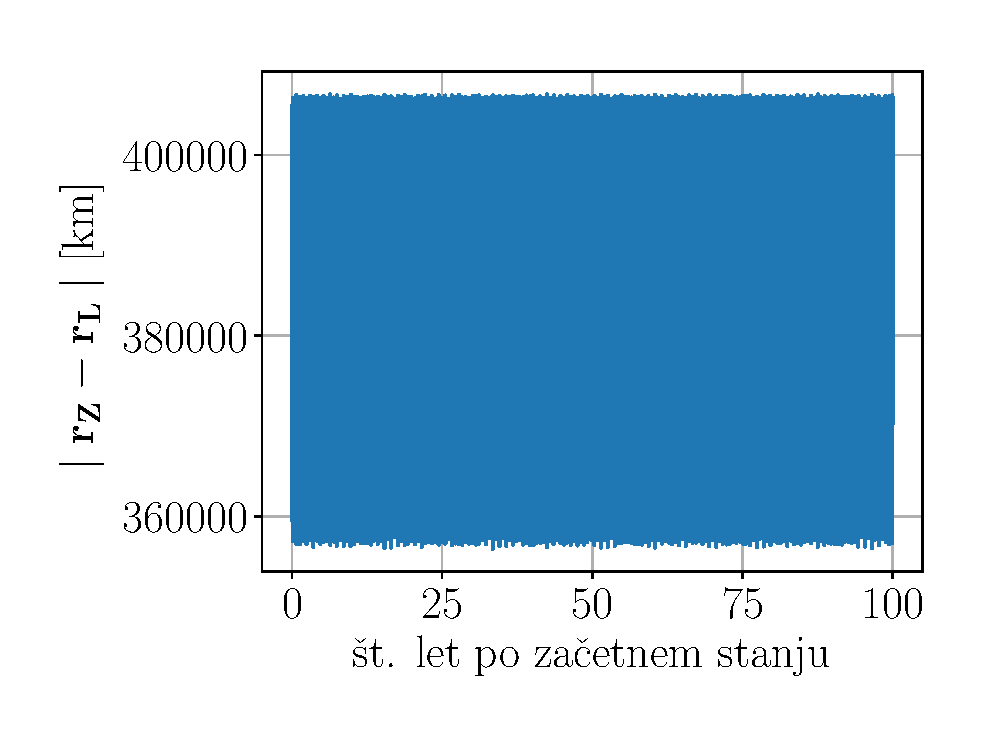
\includegraphics[scale=0.45]{slikep/razdaljaZL.eps}
        \begin{minipage}{0.75\textwidth}
            \caption{Razdalja med Zemljo in Luno.}
        \end{minipage}%
    \end{minipage}%
    \hfill
    \begin{minipage}[t]{.5\textwidth}
        \centering
        \includegraphics[scale=0.45]{slikep/razdaljaSZ.eps}
        \begin{minipage}{0.75\textwidth}
            \caption{Razdalja med Soncem in Zemljo.}
        \end{minipage}
    \end{minipage}
\end{figure}

\newpage

\subsection{Precesija vozelne črte}
\begin{figure}[h!]
    \centering
    \includegraphics[scale=0.53]{slikep/nodal-angle.eps}
    \captionof{figure}{Kot vozelne črte glede na začetno lego vozelne črte.}
    \label{fig:nodal-angle}
\end{figure}

\noindent
Periodo določimo tako, da poiščemo maksimume korelacije funkcije same s sabo
pri različnih zamikih začetnega kota.

\begin{figure}[h]
    \centering
    \begin{minipage}[t]{.65\textwidth}\vspace{0pt}%
        \centering
        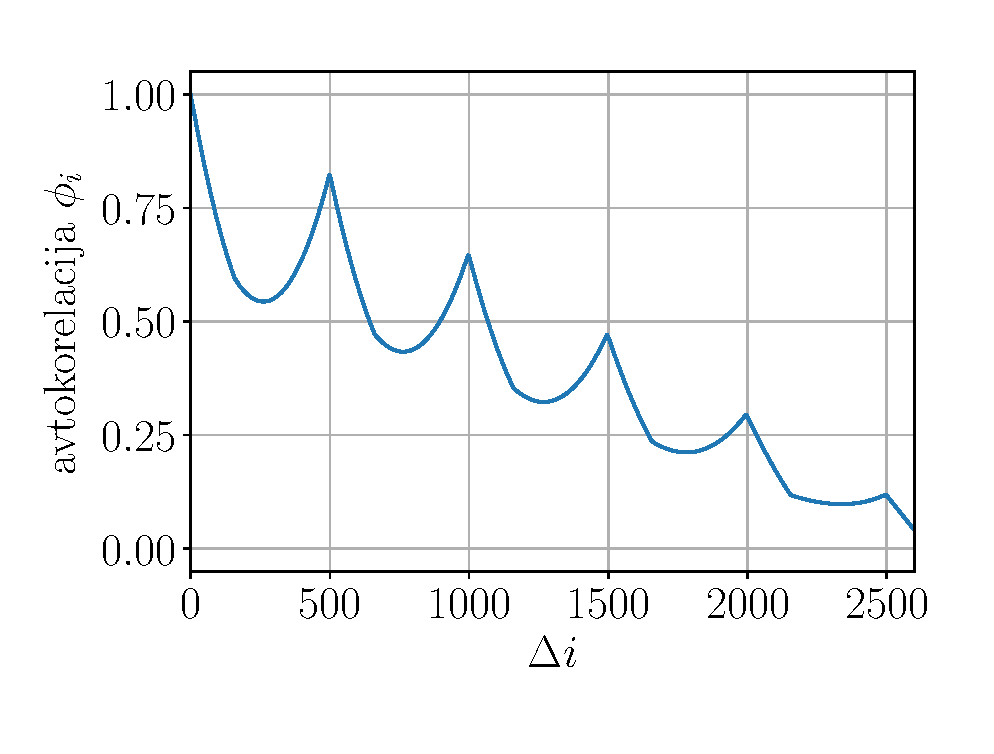
\includegraphics[scale=0.6]{slikep/nodal-angle-acorr.eps}
        \captionof{figure}{Avtokorelacija kota vozelne črte v odvisnosti od 
        zamika za $\Delta i$ kotov.}
        \label{fig:nodal-acorr}
    \end{minipage}%
    \qquad
    \begin{minipage}[t]{.28\textwidth}\vspace{4em}%
        \begin{center}
            \begin{tabular}{c c}
                \toprule
                $\Delta \max$ & $\Delta t$\ [dni] \\
                \midrule[0.03em]
                498 & 6775.88 \\
                498 & 6775.75 \\
                500 & 6802.62\\
                498 & 6775.46 \\
                500 & 6802.96 \\
                \bottomrule
            \end{tabular}
            \vspace{2.76em}
            \captionof{table}{Razdalje med maksimumi grafa in časovni intervali
            med njimi.}
        \end{center}
    \end{minipage}
\end{figure}

\noindent
Časovni intervali med maksimumi grafa \ref{fig:nodal-acorr} so približno enako
dolgi, zato izračunamo periodo kot povprečje petih period. Časovni 
interval petih period je dolg \linebreak 
$\SI{33933}{dni}\pm\SI{7}{dni}$. Povprečna 
perioda je torej $\SI{6786}{dni}\pm\SI{2}{dneva}$, kar je blizu referenčne 
vrednosti $\SI{6798.38}{dni}$~\cite{nasassd}. Del napake izvira iz tega, da smo 
izračunali kot vozelne črte le, ko je Luna prečkala ekliptiko, torej 
približno vsakih 14 dni. Časovni intervali so zato določeni z natančnostjo 
$\SI{7}{dni}$, povprečna perioda pa na $\SI{2}{dneva}$, kar še ne 
pojasni odstopanja rezultata od referenčne vrednosti v celoti. Najverjetneje 
izhaja iz tega, da nismo upoštevali oblike Zemlje in vpliva drugih teles v 
Osončju.

\noindent
Zanimivo je, da se kot vozelne črte ne spreminja povsem linearno. Če točkam
iz grafa \ref{fig:nodal-angle} znotraj prve periode odštejemo linearno 
funkcijo, ki se jim najbolj prilega, dobimo graf podoben sinusni funkciji.
Periodo nihanja hitrosti precesije vozelne črte poiščemo z avtokorelacijo.

\begin{figure}[h!]
    \centering
    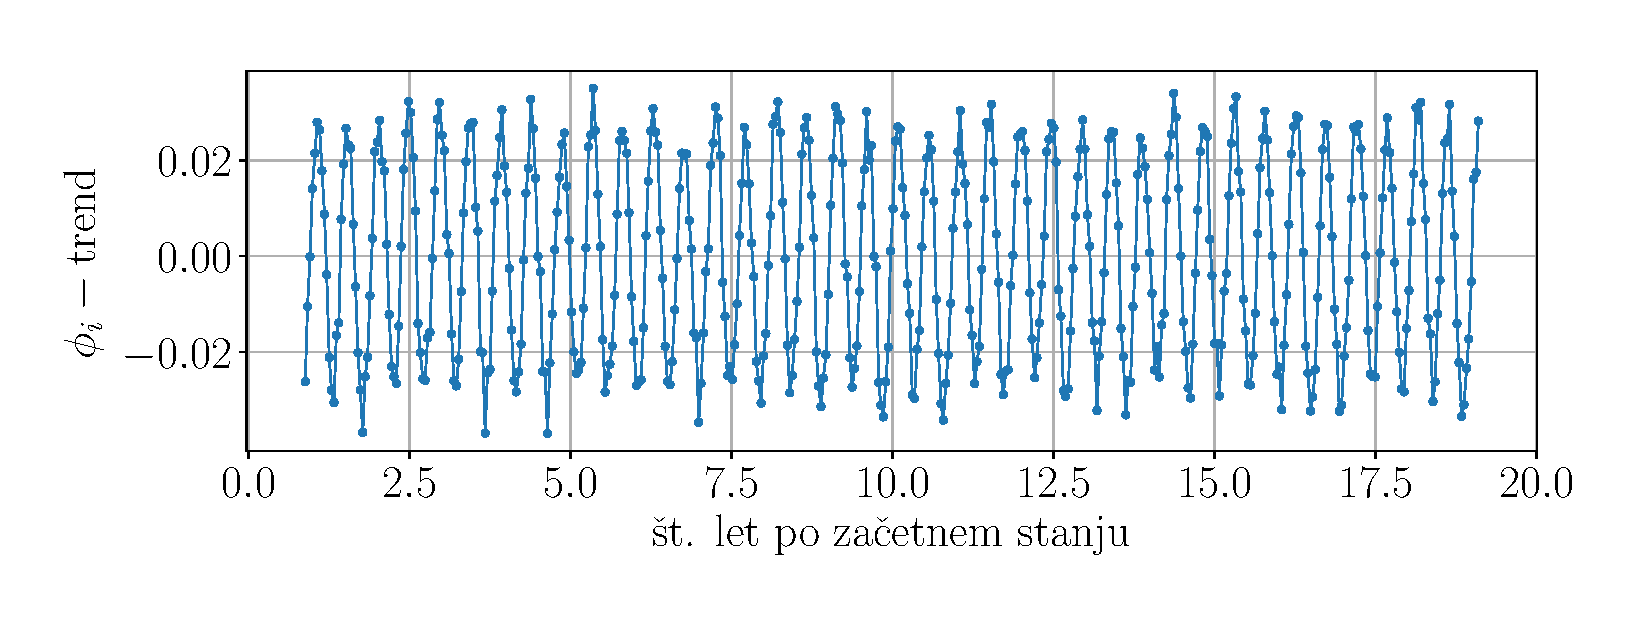
\includegraphics[scale=0.55]{slikep/nodal-angle-detrend.eps}
    \captionof{figure}{Odstopanje kota vozelne črte od linearne funkcije, ki
    se točkam najbolj prilega znotraj prve periode precesije.}
\end{figure}

\begin{figure}[h!]
    \centering
    \includegraphics[scale=0.55]{slikep/nodal-angle-detrend-acorr.eps}
    \captionof{figure}{Avtokorelacija odstopanja kota vozelne črte od 
    prilagojene linearne funkcije v odvisnosti od zamika za $\Delta i$ kotov.}
\end{figure}

\noindent
Po 38 periodah je $\Delta i = 483$, kar je $\SI{6586}{dni}\pm\SI{7}{dni}$.
Povprečna perioda je torej $\SI{173.3}{dni}\pm\SI{0.2}{dneva}$. To je približno
pol leta, zato sklepamo, da je nihanje hitrosti precesije vozelne črte 
posledica spreminjanja smeri vozelne črte glede na Sonce.

Izračunamo kot $\beta_i$ med vsakim vektorjem vozelne črte $\vec{e_i}$ in 
krajevnim vektorjem težišča sistema Zemlja-Luna $\vec{r_T}$ ob istem času. 
Uporabimo podobno formulo kot za kot vozelne črte~\eqref{eq:nodal-kot}
\begin{equation*}
    \beta_i = \left\{
        \begin{array}{ll}
            \arccos{\frac{\: \vec{r_T} \cdot \vec{e_i}}
            {\; \norm{\vec{r_T}} \ \norm{\vec{e_i}}}} & 
            {;\ (\vec{r_T}\times\vec{e_i})\cdot\vec{n} \geq 0} \vspace{0.5em} \\
            2\pi - \arccos{\frac{\: \vec{r_T} \cdot \vec{e_i}}
            {\; \norm{\vec{r_T}} \ \norm{\vec{e_i}}}} & 
            {;\ (\vec{r_T}\times\vec{e_i})\cdot\vec{n} < 0}
        \end{array}
    \right.
\end{equation*}

\newpage

\begin{figure}[h!]
    \centering
    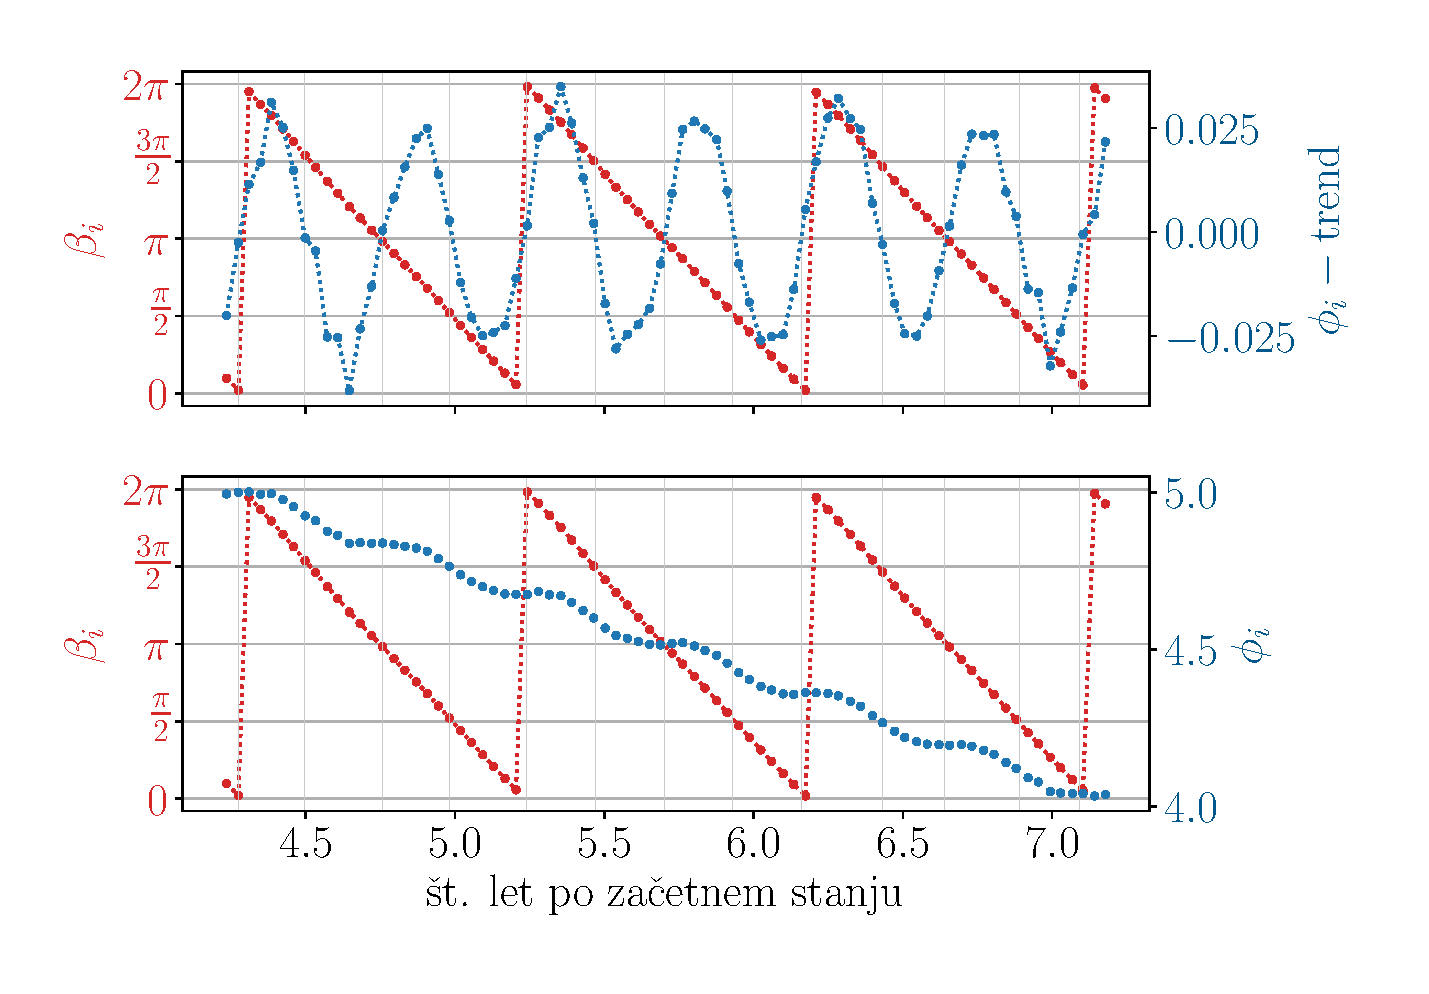
\includegraphics[scale=0.59]{slikep/nodal-angle-comp.eps}
    \captionof{figure}{Zgoraj: Z rdečo kot med vektorjem vozelne črte in 
    krajevnim vektorjem težišča sistema Zemlja-Luna in z modro razlika med 
    kotom vozelne črte in prilagojeno premico. Spodaj: Z rdečo kot med 
    vektorjem vozelne črte in krajevnim vektorjem težišča sistema Zemlja-Luna 
    in z modro kot vozelne črte.}
    \label{fig:nodal-angle-comp}
\end{figure}

\noindent
Na zgornjem grafu na grafu \ref{fig:nodal-angle-comp} opazimo, da je perioda 
$\beta_i$ ravno dvakrat daljša od periode $\phi_i-\mathrm{trend}$, kar kaže, da
je hitrost precesije vozelne črte povezana s smerjo vozelne črte glede na Sonce.

Ko je kot $\beta_i$ blizu $0$ ali $\pi$, je 
eden od vozlov med Soncem in Zemljo. Na spodnjem grafu vidimo, da se takrat kot 
vozelne črte ne spreminja opazno. Ko je kot $\beta$ enak $\frac{\pi}{2}$ ali 
$\frac{3\pi}{2}$ je vozelna črta pravokotna na krajevni vektor težišča. Tedaj 
je naklon grafa $\phi_i$ največji in se smer vozelne črte najhitreje spreminja. 

Poskusimo razložiti opaženo odvisnost na grafu. Do precesije vozelne črte pride 
zaradi navora tiste komponente gravitacijske sile Sonca, ki je pravokotna na 
ravnino Lunine tirnice. 

Ko je kot $\beta$ blizu $\frac{\pi}{2}$ ali $\frac{3\pi}{2}$ (slika 
\ref{fig:sile-nodal-iste}), kaže pravokotna komponenta v obeh delih tirnice 
(nad in pod ekliptiko) v isto smer. Zato se v bližini teh kotov učinka sil v 
obeh delih seštejeta in je hitrost precesije največja.

\renewcommand{\figurename}{Slika}

\begin{figure}[h!]
    \centering
    \includegraphics[scale=1.4]{slikep/nodal-max.png}
    \captionof{figure}{Sile na Luno pri kotu vozelne črte $\frac{\pi}{2}$ 
    in $\frac{3\pi}{2}$ v obeh delih orbite. Z rdečo barvo sili na Luno, z 
    vijolično barvo komponenti, ki sta pravokotni na ravnino Lunine tirnice, 
    z modro pa ostali komponenti. Ni v merilu.}
    \label{fig:sile-nodal-iste}
\end{figure}

\newpage

\noindent
Ko je kot $\beta$ blizu $0$ ali $\pi$ (slika \ref{fig:sile-nodal-razlicne}), 
kaže pravokotna komponenta v delu tinice pod ekliptiko v eno smer, v delu 
tirnice nad ekliptiko pa v nasprotno smer. Zato v bližini teh kotov učinek 
sile na enem delu tirnice skoraj povsem izniči učinek sile na drugem delu in je 
hitrost precesije najmanjša.

\begin{figure}[h!]
    \centering
    \includegraphics[scale=1.2]{slikep/nodal-min.png}
    \captionof{figure}{Sile na Luno pri kotu vozelne črte $0$ in $\pi$ v obeh
    delih orbite. Z rdečo barvo sili na Luno, z vijolično barvo komponenti, 
    ki sta pravokotni na ravnino Lunine tirnice, z modro pa ostale komponente. 
    Ni v merilu.}
    \label{fig:sile-nodal-razlicne}
\end{figure}

\renewcommand{\figurename}{Graf}

\newpage

\subsection{Precesija dolge osi}

\begin{figure}[h!]
    \centering
    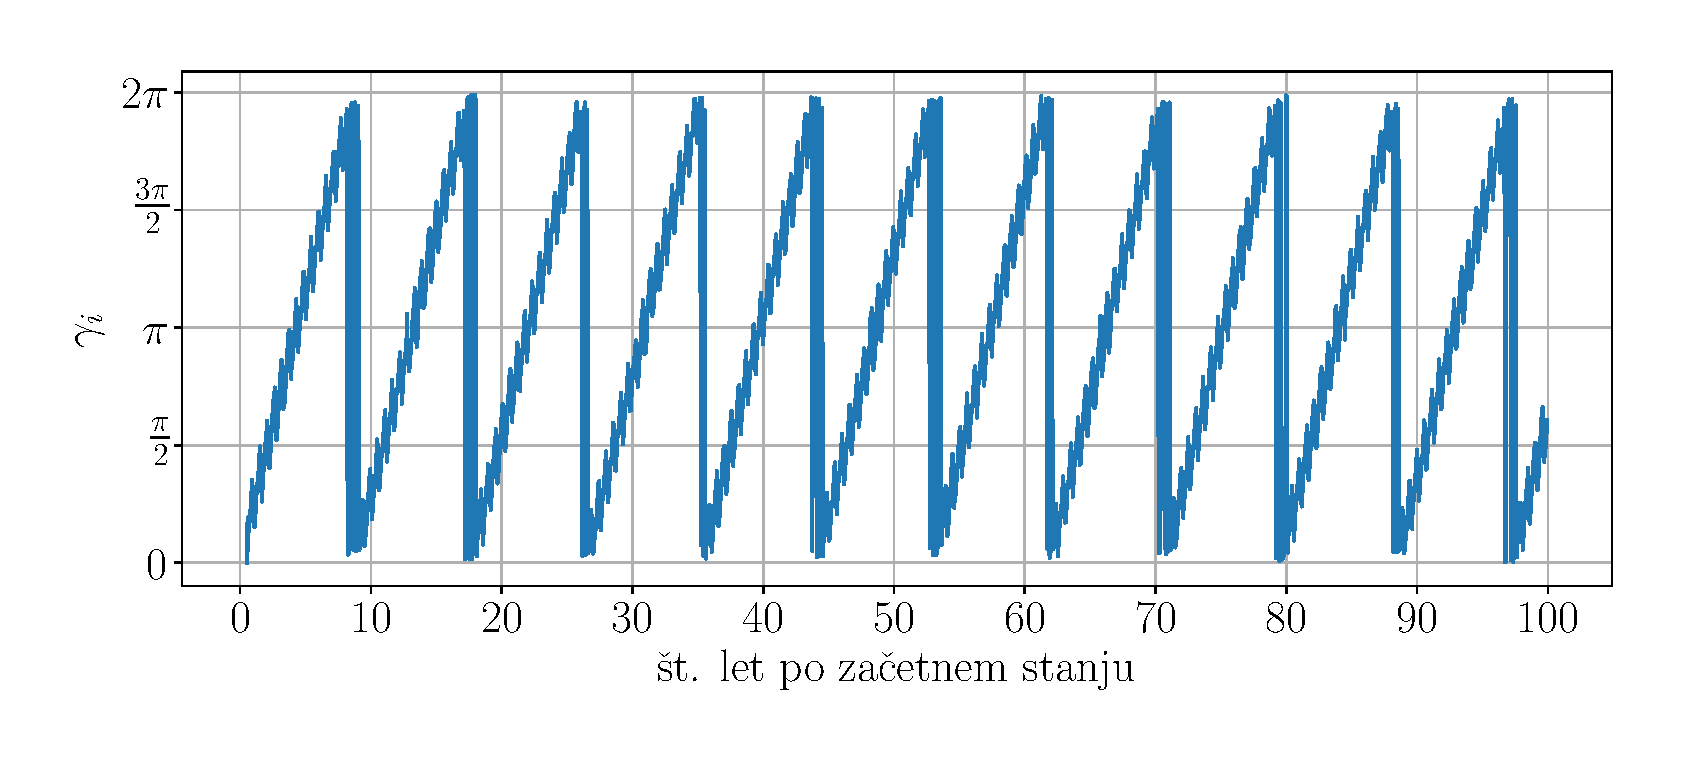
\includegraphics[scale=0.53]{slikep/apsidal-angle.eps}
    \captionof{figure}{Kot dolge osi glede na začetno lego dolge osi.}
    \label{fig:apsidal-angle}
\end{figure}

\noindent
Graf kota dolge osi je podoben grafu kota vozelne črte, le da je perioda
krajša in se dolga os vrti v drugo smer. Periodo določimo z avtokorelacijo.

\begin{figure}[h]
    \centering
    \begin{minipage}[t]{.66\textwidth}\vspace{1pt}%
        \centering
        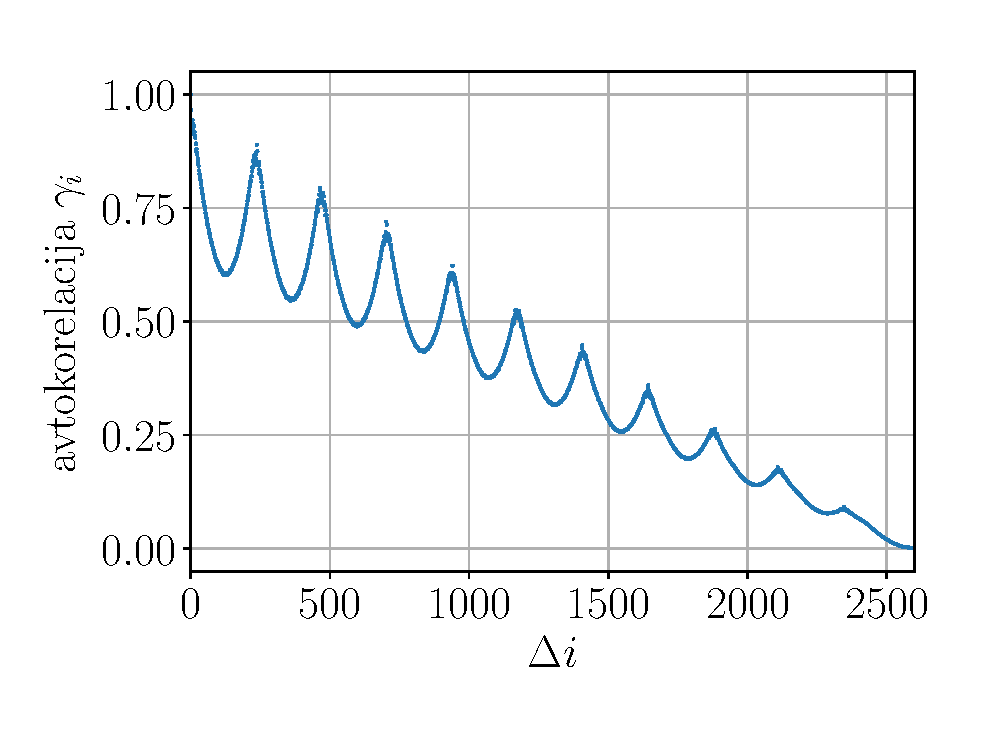
\includegraphics[scale=0.6]{slikep/apsidal-angle-acorr.eps}
        \captionof{figure}{Avtokorelacija kota dolge osi od v odvisnosti od 
        zamika za $\Delta i$ kotov.}
        \label{fig:apsidal-acorr}
    \end{minipage}%
    \qquad
    \begin{minipage}[t]{.27\textwidth}\vspace{7.7pt}%
        \begin{center}
            \begin{tabular}{c c}
                \toprule
                $\Delta \max$ & $\Delta t$\ [dni] \\
                \midrule[0.03em]
                236 & 3254.71 \\
                235 & 3235.79 \\
                233 & 3209.04 \\
                235 & 3239.17 \\
                235 & 3239.04 \\
                235 & 3236.58 \\
                235 & 3235.50 \\
                234 & 3227.46 \\
                234 & 3221.83 \\
                235 & 3238.29 \\
                \bottomrule
            \end{tabular}
            \captionof{table}{Razdalje med maksimumi grafa in časovni intervali
            med njimi.}
        \end{center}
    \end{minipage}
\end{figure}

\noindent
Časovni intervali med maksimumi grafa \ref{fig:apsidal-acorr} so približno 
enako dolgi, zato \linebreak 
izračunamo periodo kot povprečje desetih period. Časovni interval desetih 
period je $\SI{32322}{dni}\pm\SI{7}{dni}$. Povprečna perioda je torej 
$\SI{3232}{dni}\pm\SI{1}{dan}$, kar je v okviru napake enako 
referenčni vrednosti $\SI{3231.50}{dni}$~\cite{nasassd}.

Tako kot kot vozelne črte, se tudi kot dolge osi ne spreminja povsem linearno.
Če točkam iz grafa \ref{fig:apsidal-angle} znotraj prve periode odštejemo
linearno funkcijo, ki se jim najbolj prilega, dobimo graf podoben sinusni 
funkciji. Periodo nihanja hitrosti precesije dolge osi določimo z 
avtokorelacijo.

\newpage

\begin{figure}[h!]
    \centering
    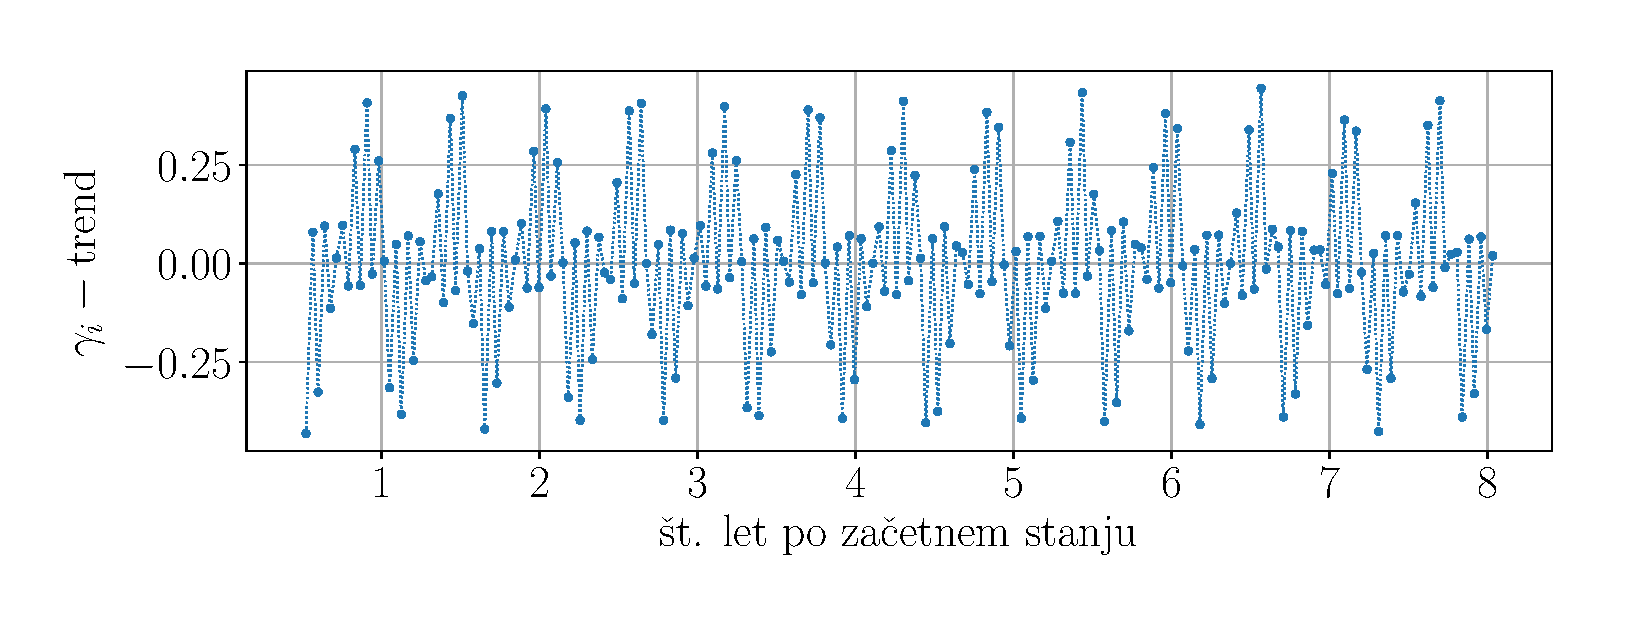
\includegraphics[scale=0.55]{slikep/apsidal-angle-detrend.eps}
    \captionof{figure}{Odstopanje kota dolge osi od linearne funkcije, ki
    se točkam na grafu \ref{fig:apsidal-angle} najbolj prilega znotraj prve 
    periode precesije.}
\end{figure}

\begin{figure}[h!]
    \centering
    \includegraphics[scale=0.55]{slikep/apsidal-angle-detrend-acorr.eps}
    \captionof{figure}{Avtokorelacija odstopanja kota vozelne črte od 
    prilagojene linearne funkcije v odvisnosti od zamika za $\Delta i$ kotov.}
\end{figure}

\noindent
Po 13 periodah je $\Delta i = 194$, kar je $\SI{2676}{dni}\pm\SI{7}{dni}$.
Povprečna perioda je torej $\SI{205.9}{dni}\pm\SI{0.5}{dneva}$. To je približno
pol leta, zato sklepamo, da je nihanje hitrosti precesije dolge osi posledica
spreminjanja smeri dolge osi glede na Sonce.

Izračunamo kot $\tau_i$ med vsakim vektorjem dolge osi $\vec{f_i}$ in 
krajevnim vektorjem težišča sistema Zemlja-Luna $\vec{r_T}$ ob istem času. 
Uporabimo podobno formulo kot za kot vozelne črte~\eqref{eq:nodal-kot}

\begin{equation*}
    \tau_i = \left\{
        \begin{array}{ll}
            \arccos{\frac{\: \vec{r_T} \cdot \vec{f_i}}
            {\; \norm{\vec{r_T}} \ \norm{\vec{f_i}}}} & 
            {;\ (\vec{r_T}\times\vec{f_i})\cdot\vec{n} \geq 0} \vspace{0.5em} \\
            2\pi - \arccos{\frac{\: \vec{r_T} \cdot \vec{f_i}}
            {\; \norm{\vec{r_T}} \ \norm{\vec{f_i}}}} & 
            {;\ (\vec{r_T}\times\vec{f_i})\cdot\vec{n} < 0}
        \end{array}
    \right.
\end{equation*}

\newpage

\begin{figure}[h!]
    \centering
    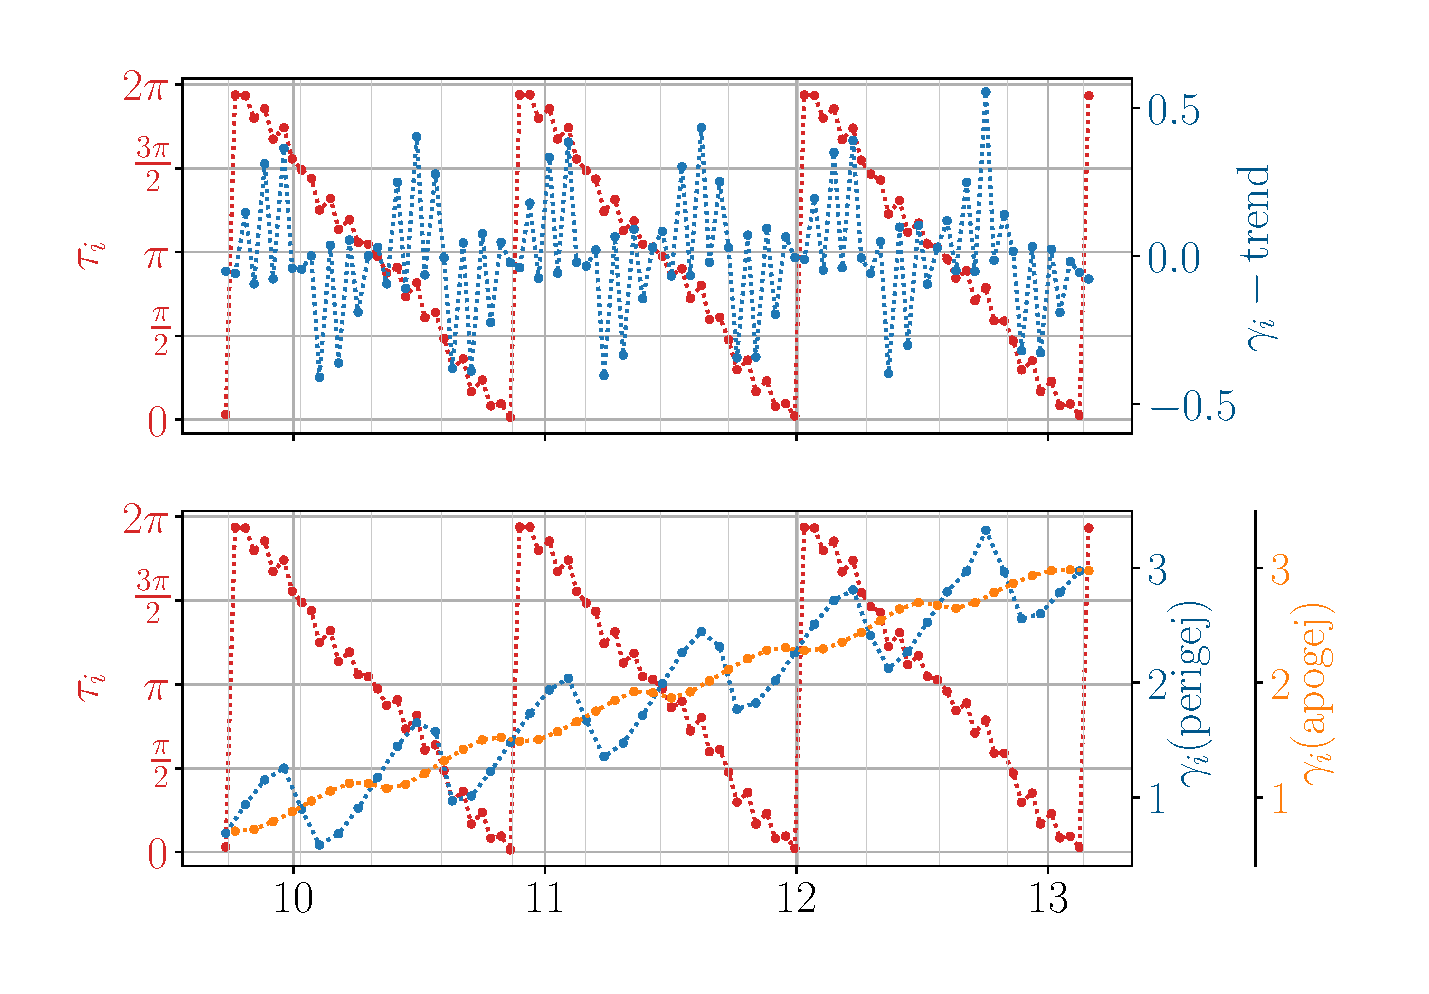
\includegraphics[scale=0.57]{slikep/apsidal-angle-comp.eps}
    \captionof{figure}{Zgoraj: Z rdečo kot med vektorjem dolge osi in 
    krajevnim vektorjem težišča sistema Zemlja-Luna in z modro razlika med 
    kotom dolge osi in prilagojeno premico. Spodaj: Z rdečo kot med vektorjem 
    dolge osi in krajevnim vektorjem težišča sistema Zemlja-Luna, z modro kot 
    dolge osi izračunan iz perigejev in z rumeno kot dolge osi izračunan iz 
    apogejev.}
    \label{fig:apsidal-angle-comp}
\end{figure}

\noindent
Na zgornjem grafu na grafu \ref{fig:apsidal-angle-comp} opazimo, da je perioda
$\tau_i$ ravno dvakrat daljša od periode $\gamma_i-\mathrm{trend}$, kar kaže, 
da je hitrost precesije dolge osi povezana s smerjo dolge osi glede na Sonce.

Ko je kot $\tau_i=0$, je Lunin perigej med Soncem in Zemljo, ko je $\tau_i=\pi$ 
pa je med Sonce in Zemljo apogej. Iz spodnjega grafa vidimo, da se pri teh dveh 
kotih apogej ne spreminja opazno, kot perigeja pa prehiti kot apogeja.  Ko je 
$\tau_i$ enak $\frac{\pi}{2}$ ali $\frac{3\pi}{2}$, je dolga os 
pravokotna na krajevni vektor težišča. Tedaj je naklon grafa kota dolge osi, 
določenega z apogeji, največji in se apogej najhitreje spreminja, kot določen
s perigeji pa se manjša. Opazimo, da se kota dolge osi, določena iz apogeja in 
perigeja, približno ujemata pri $\tau=0,\frac{\pi}{2},\pi,\frac{3\pi}{2}$.

Poskusimo razložiti opaženo odvisnost na grafu. Do precesije dolge osi pride 
zaradi radialne in tangentne komponente gravitacijske sile Sonca. 
Na grafu opazimo, da se kot perigeja ob nekaterih trenutkih razlikuje od
kota apogejev. To je mogoče, ker se tekom enega obhoda Lune tirnica spreminja
zaradi vpliva radialne in tangentne komponente sile Sonca.
Na poti Lune od apogeja do perigeja se lahko tirnica zavrti v smeri ure in Luna 
zato doseže perigej prej kot v prejšnji orbiti. Kot perigeja se zato lahko 
zmanjša. V drugi polovici orbite se tirnica zasuka nazaj, zato lahko kot 
apogeja ostane približno enak oz. se celo poveča. To se zgodi, ko je \linebreak
$\tau_i$ blizu $\frac{\pi}{2}$ in $\frac{3\pi}{2}$. V bližini $0$ in $\pi$ pa
se tirnica zavrti v nasprotni smeri ure in Luna doseže perigej pozneje kot v
prejšnji orbiti in se kot perigeja veča. Kota dolge osi, določena iz 
apogeja in perigeja se približno ujemata v bližini večkratnikov 
$\frac{\pi}{2}$, ker se tedaj učinka sile Sonca v posameznih polovicah orbite 
skoraj povsem izničita. 

\newpage
\begin{thebibliography}{1}
    \bibitem{apsidal} Shkelzen Cakaj,  Bexhet Kamo, Algenti Lala,
    Ilir Shinko \& Elson Agastra. \textit{The Apsidal Precession for Low Earth 
    Sun Synchronized Orbits.} International Journal of Advanced Computer 
    Science and Applications. 6. 10.14569/IJACSA.2015.060909. (2015)
    \bibitem{nasassd} Solar System Dynamics Group, 
    Horizons On-Line Ephemeris System, \\ 
    \url{https://ssd.jpl.nasa.gov/horizons.cgi}. Pridobljeno 7. 7. 2019.
    \bibitem{nodal} Sandra Matthews. \textit{Phases of the Moon. Spin and 
    orbital frequencies.} \\
    \url{https://slideplayer.com/slide/6237929/}
    \bibitem{odeint} SciPy v1.3.0, scipy.integrate.odeint,
    \url{https://docs.scipy.org/doc/scipy/reference/generated/scipy.integrate.
    odeint.html}
    \bibitem{repo} \url{https://gitlab.com/rokuk/sim-precesija-lune}
    \bibitem{konstante} William M. Folkner, James G. Williams, Dale H. Boggs, 
    Ryan S. Park, \& Petr Kuchynka. \textit{The Planetary and Lunar Ephemerides 
    DE430 and DE431.} The Interplanetary Network Progress Report, Volume 42-196, 
    (2014). 
    \mbox{\url{https://ipnpr.jpl.nasa.gov/progress_report/42-196/196C.pdf}}
    \bibitem{codata} P. J. Mohr, D. B. Newell \& B. N. Taylor, \textit{CODATA 
    recommended values of the fundamental physical constants: 2014.} Journal of 
    Physical and Chemical Reference Data 45(4), 043102 (2016).
    \url{https://arxiv.org/abs/1507.07956}
\end{thebibliography}

\end{document}
